\section{Les dispositifs expérimentaux}
Dans cette section, nous allons introduire les deux dispositifs expérimentaux conçu pour la caractérisation des modules optiques (OMs) d'AMANDA.

\subsection{Dispositif 1: Effet Tcherenkov par des électrons}

Cette manipulation utilise une source de radiation $\beta^+$ composée de Strontium $^{90}$Sr. Les électrons émis par la source traverse ensuite une plaque de quartz d'indice de réfraction  $n = 1.478$. Lors de leur passage, les électrons vont produire un rayonnement Tcherenkov qui pourra être détecté par l'OM. Dans ce dispositif, l'OM se trouve à une position fixe située à un angle de 45$^{\circ}$ par rapport à la direction d'émission des électrons. La source radioactive est combinée à un spectromètre qui va nous permettre de sélectionner l'énergie cinétique des électrons afin de récolter un maximum de rayonnement Tcherenkov dans l'OM. Pour déterminer l'intensité du courant à fournir au spectromètre pour obtenir des électrons de cette énergie, vous devrez d'abord résoudre l'exercice 2.\\

Une fois cette valeur trouvée, vous pouvez allumer le spectromètre. Ce spectromètre est calibré sur la partie descendante de la courbe d'hystérèse, il vous faudra donc respecter les conditions d'utilisations décrites ci-dessous.\\

\textbf{Mode d'emploi du spectromètre :}
\begin{quote}
    \begin{itemize}
        \item Démarrez à $I$ = 0 A
        \item Aller à saturation $I$ $\sim$ 2,6 A
        \item Descendre à la valeur $I_t$ désirée
    \end{itemize}
\end{quote}
\textbf{Remarque :} Si on veut changer $I_t$ pour une valeur plus petite, on descend vers cette valeur. En revanche, si on veut augmenter cette valeur, on doit recommencer le cycle d'hystérèse. 

\begin{figure}[!h]
    \center{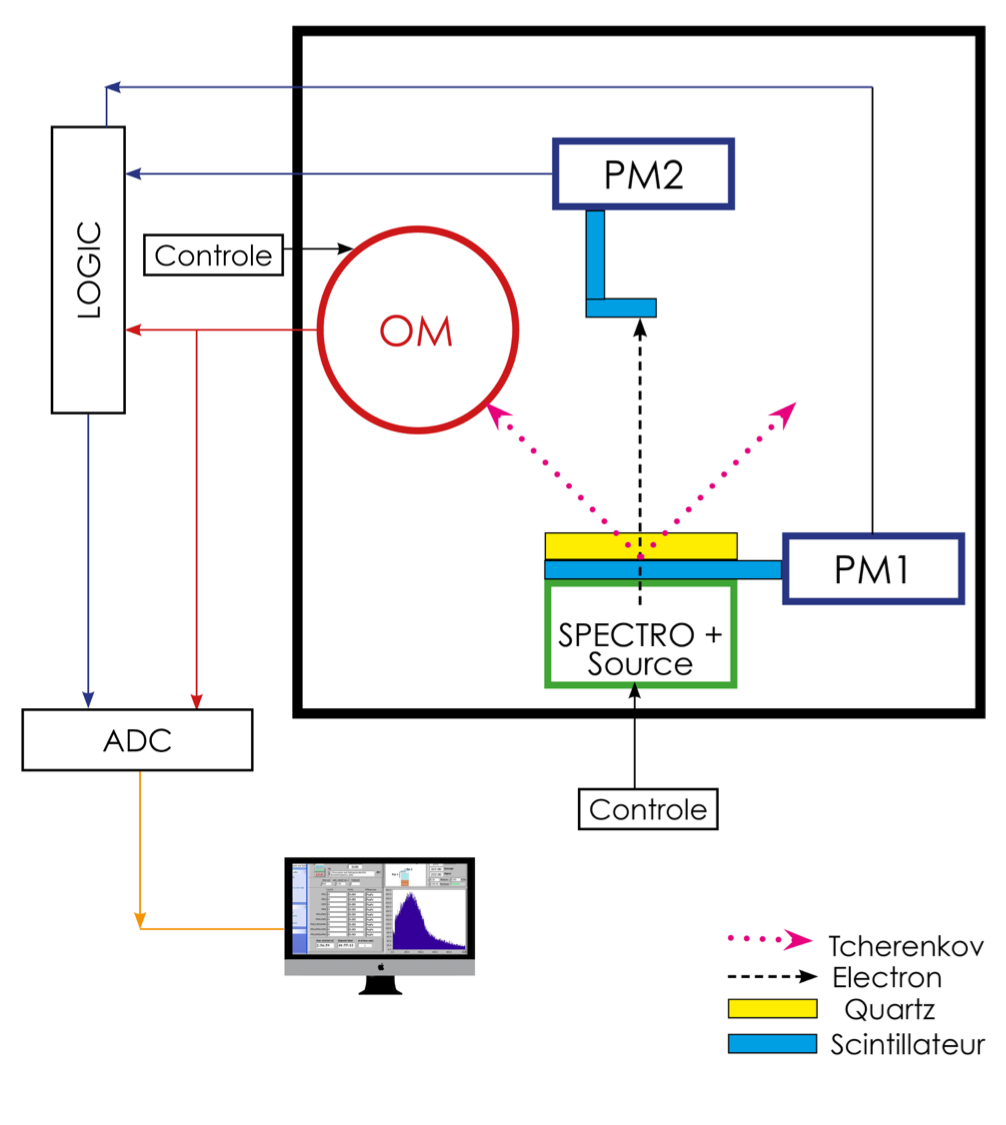
\includegraphics[width=0.5\textwidth]
    {figures/Dispositif_1.png}}
    \caption{\label{fig:dispo1} Dispositif expérimental de l'effet Tcherenkov produit par des électrons.}
\end{figure}

Dans ce dispositif, sont également présent 2 photo-multiplicateurs (PMs) chacun relié à un scintillateur. Le premier (PM1) est situé entre la source et la plaque de quartz et nous permet de vérifier qu'un électron a été émis par la source. Le second PM confirme que l'électron a bien traversé le quartz. Ces PMs ont donc pour but d'assurer que le signal détecté par l'OM est en coïncidence avec un électron qui a produit des photons Tcherenkov.

\subsection{Dispositif 2: Effet Tcherenkov par des muons}

Pour cette seconde manipulation, nous utilisons les muons atmosphériques afin d'obtenir l'émission Tcherenkov. Ce dispositif est composé de 4 scintillateurs chacun relié à un photo-multiplicateur (PM), d'un OM, une couche de plomb et d'un réservoir d'eau. Ce réservoir forme un angle de 45$^{\circ}$ avec la verticale. Les trois premiers PM (PM1, PM2 et PM3) assure la direction verticale du muon incident. La présence d'une couche de plomb avant le PM3 nous permet également de vérifier que le muon est suffisamment énergétique pour produire le rayonnement Tcherenkov avec l'angle souhaité. Un 4ème PM est placé au dessus de l'OM et est utilisé comme veto. Puisque les muons sont produits en "paquets", appelés muon bundles, ce veto exclu les évènements de l'OM qui seraient produits par un second muon plutôt que par un photon Tcherenkov.


\begin{figure}[!h]
    \center{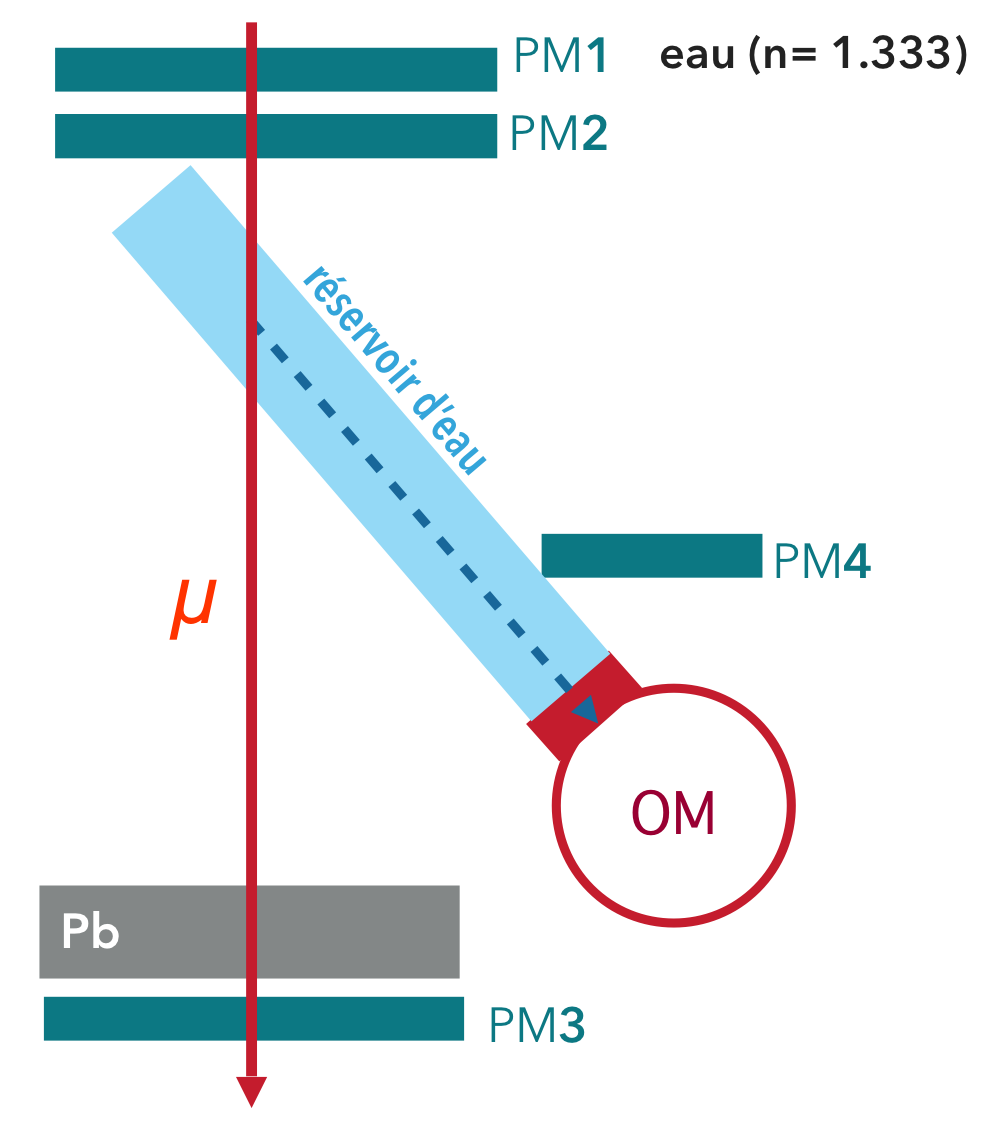
\includegraphics[width=0.5\textwidth]
    {figures/Dispositif_2.png}}
    \caption{\label{fig:dispo2} Dispositif expérimental de l'effet Tcherenkov produit par des muons.}
\end{figure}


\subsection{Le matériel expérimental}


\pagebreak